
\section{Objective}

The purpose of this experiment is to determine the magnetic moment of a free electron.
To implement this the electronspin-resonance is used.


\section{Theory}
In quantum mechanics the status of particles is described by a wave function.
\begin{equation*}
  \psi_{n,l,m}(r,\theta,\phi) = R_{n,l}(r) \cdot \Theta_{l,m}(\theta) \cdot \Phi_m(\phi)
\end{equation*}
Thereby r is the radial part, $\Theta$ discribes the polar angle and
$\Phi$ is the part of the azimuth angle.
N, l, m are quantum numbers.
N is the principal quantum number and describes the energy level.
L is the number of the orbital angular momentum.
M characterises the orientation of the system and can take the values 2l+1.

The current density is defined by
\begin{equation*}
  S = \frac{\hbar}{2im_0}\cdot (\psi* \nabla \psi - \psi \nabla \psi* ).
\end{equation*}
It results of moving electrons on the shell of an atom which implies a magnetic moment
\begin{equation*}
  \mu_z =\mu_b \cdot m,
\end{equation*}
with $\su{\mu_b}$ the Bohr magneton.
Figure \ref{fig:muz} shows the geometric thoughts to deduce the magentic moment.
\begin{figure}[H]
  \centering
  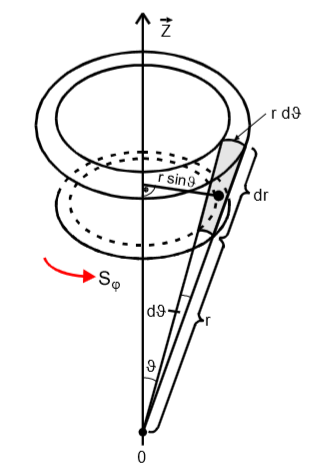
\includegraphics[scale=0.6]{pictures/1.png}
  \caption{derivation of the magnetic moment \cite{anleitung}}
  \label{fig:muz}
\end{figure}
In a homogeneous magnetic field the magnetic momentum of the electron shell is
connected to the outer magnetic field.
The quantization of the direction leads to the zeeman-effect,
which describes the split of the energy levels in the outer magnetic field.
It is shown in figure \ref{fig:eniveau}.
\begin{figure}[H]
  \centering
  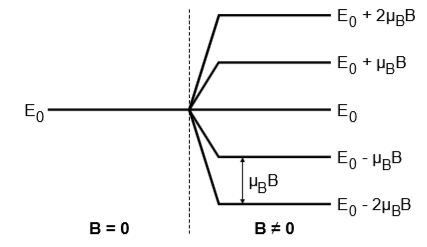
\includegraphics[scale=0.6]{pictures/2.png}
  \caption{Split of the energy niveau \cite{anleitung}}
  \label{fig:eniveau}
\end{figure}
A split of an electron without orbital angular momentum is not expected.
In the Stern-Gerlach-experiment the split of the electron into two resulting beams in a inhomogeneous
magnetic field leads to the postulate of the existence of another angular moment, which is
called spin.
The electron is a fermion and has the spin  $|S| = \sfrac{1}{2}$.
The z-component of the magnetic moment is able to take two directions which are determined by
the quantum number $m_s \in [-1/2, 1/2]$. The relation between spin and related magnetic moment is
often expressed in the unit of the bohr magneton
\begin{equation*}
  \mu_{sz} = -gm_s\mu_B.
\end{equation*}
The energy difference between two niveaus
\begin{equation*}
  \Delta E = g\mu_B B
\end{equation*}
is needed to get the electrons into a higher energy level. G the gyromagnetic relation or Landé-factor.

In thermal equilibrium the two energy levels are filled according to the Boltzmann-statistic.
By a large number of electrons the upper level is less filled than the lower one.
The Energy $\su{\Delta E}$ is given to the system by inserting high frequenzy HF-quantum.
Because of this elctrons are able to go from the lower level to the upper.
Therefore the electrons' spin is flipped. This methode of transporting electrons into a
higher level of energy by flipping the spin is called the electronspin-resonance.

\section{Experimental setup}
The experimental setup is presented in figure \ref{fig:aufbau}.
\begin{figure}
  \centering
  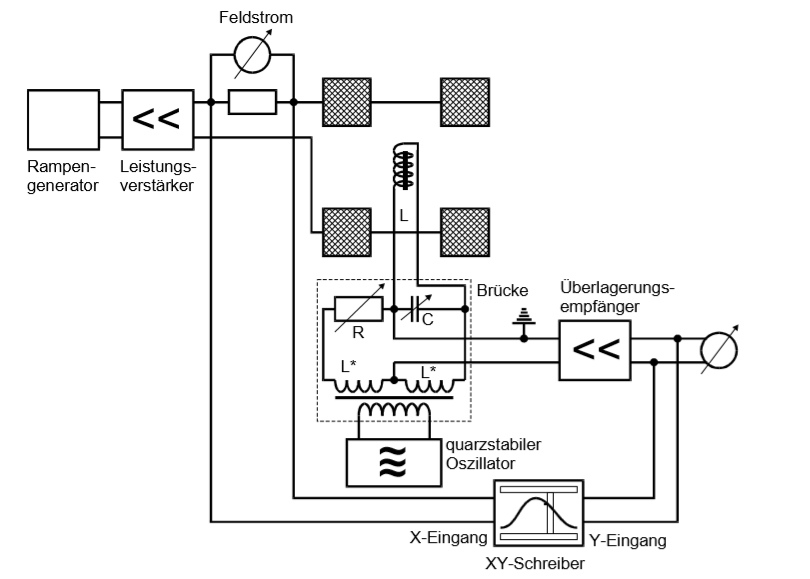
\includegraphics[scale=0.6]{pictures/5.png}
  \caption{construction of the experiment \cite{anleitung}}
  \label{fig:aufbau}
\end{figure}
As a sample Diphenylpikrylhydeazyl with its chemical structure of one free electron is used.
This sample is located in the HF-coil. The coil is supplied with current of a quarstable HF-generator and connected
with them over a bridge circuit. The variable elements R, $\su{C_{grob}}$ and $\su{C_{fein}}$ are needed
to adjust the bridge voltage. Through an overlap receiver the interference voltage is suppressed
and the bridge voltage amplified. \newline
The first amplifier enhances the input signal and also suppresses the interference voltage.
Because of the voltage generated by the Oszillograph the two signals overlab.
The following HF-amplifier supplies the highest part of amplification and inhibition of the unwanted frequencies.
The voltage with frequencies near the signal-frequency $\nu_e$ can not be inhibated completely.
to measure the alternating voltage it has to get commutated by the Demodulator.
An amplifier circuit is shown in figure \ref{fig:verstärker}.
\begin{figure}[H]
  \centering
  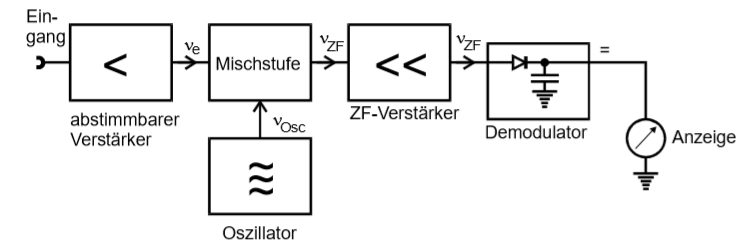
\includegraphics[scale=0.6]{pictures/6.png}
  \caption{circuit of the overlay intensifier \cite{anleitung}}
  \label{fig:verstärker}
\end{figure}
The electricity of the field coil is changing by manual interaction.
Because of this the sample is located in a changing homogeneous magnetic field which effects the Zeeman-split.
A change of the complex resistance on an arm of the bridge results in a reached response field intensity.
An other result is the high frequency bridge voltage which is addes by in a voltage amplifier.
Whith the XY-writer the resonance-curves can be drawn.
How it has to look is shown in figure \ref{fig:resonanz}
\begin{figure}[H]
  \centering
  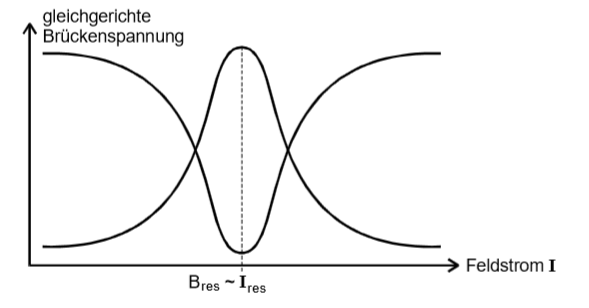
\includegraphics[scale=0.6]{pictures/7.png}
  \caption{theoretical resonace curve \cite{anleitung}}
  \label{fig:resonanz}
\end{figure}
\section{Provision}

First the bridge circuit has to be synchronized and the amplifier equipment must be set to the signal-frequency $\nu_e$.
The Oszillator-frequence $\nu_{osz}$ has to be adjust to
\begin{equation*}
  \nu_e = \nu_{osz} +\nu_{ZF}
\end{equation*}
The ZF-amplifier has to get minimized and the preamplifier has to get maximized.
After that the bridge ist going to synchronized by adjust $C_{grob}$, $C_{fein}$ and R to get a minimized signal.
Next we had to adjust the voltage to the point we could see the resonance curves.
Now the resonance curves can be drawn by the XY-writer.
Is the resonace point not located in the magnetic field it is possible to move the measuring range by the outer magnetic field.
To calculate zhe magnetic field the formula
\begin{equation}
  B(r) =\frac{8}{\sqrt{125}}v_0\frac{n}{r}I
  \label{eqn:1}
\end{equation}
is used.
Here is n = 156 and r = 0.1m.
The measuring is rerunning for four frequencies and for each frequency two times.
For the second measurement the polarity of the magnetic field is reversed.
